\documentclass{article}
% Comment the following line to NOT allow the usage of umlauts
\usepackage[utf8]{inputenc}

\usepackage{amsfonts, amsthm, amsmath, braket} 
\usepackage{tikz}
\usetikzlibrary{angles, quotes, calc, patterns}
\definecolor{cadetgrey}{rgb}{0.57, 0.64, 0.69}
% Uncomment the following line to allow the usage of graphics (.png, .jpg)
%\usepackage{graphicx}


% Start the document
\begin{document}

% Create a new 1st level heading

For orthogonal
\[
c^2 = a^2 + b^2
\]

For any obtuse 

\[
c^2 = a^2 + b^2 + 2ad
\]

dimana $d$ adalah proyeksi $b$ pada $a$.

Komposisi dari Komponen - komponen dengan Titik Aplikasi Bersama.

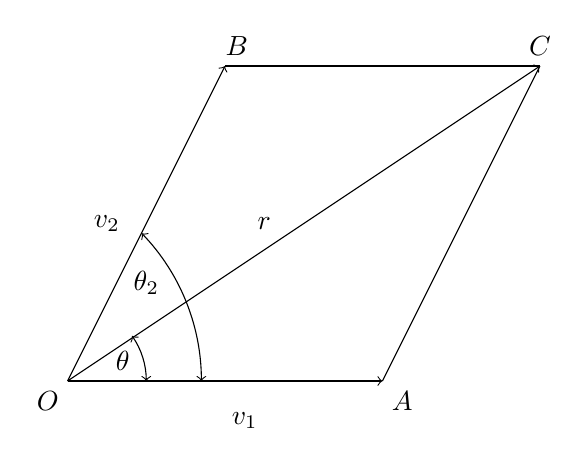
\begin{tikzpicture}
%the vectors
\draw [->, black] (1.0,0) -- (5.0,0.0);
\draw [black] (3.25, -0.5) node [black]{$v_1$};

\draw [->, black] (1.0,0) -- (3.0,4.0);
\draw (1.5, 2.0) node [black]{$v_2$}; 
\draw [black, <->] (2.7,0) arc (0:44:2.7); 
\draw (2., 1.25) node {$\theta_2$};

%the shadow
\draw [-, black] (5.0, 0,0) -- (7.0,4.0);
\draw [-, black] (3.0,4.0) -- (7.0,4.0);

%the resultant
\draw [->, black] (1.0,0) -- (7.0,4.0);
\draw [black] (3.5, 2.0) node [black]{$r$}; 
\draw [black, <->] (2.0,0) arc (0:35:1);
\draw (1.7, .25) node {$\theta$};

\draw [black] (.75, -.25) node {$O$}; 
\draw [black] (5.25, -.25) node {$A$}; 
\draw [black] (3.15, 4.25) node {$B$}; 
\draw [black] (7.0, 4.25) node {$C$}; 
\end{tikzpicture}

\begin{align*}
OA &= v_1/0 \\
OB &= v_2/\theta_2\\
OC &= r/\theta\\
r^2 &= v_1^2 + v_2^2 + 2v_1v_2\cos\theta\\
\tan\theta &= \frac{v_2\sin\theta_2}{v_1 + v_2\cos\theta_2};
\end{align*}

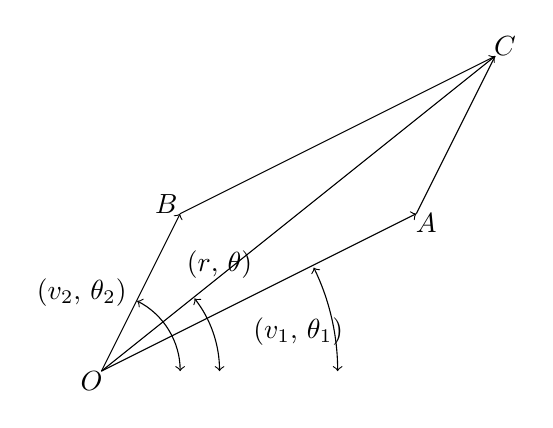
\begin{tikzpicture}
%common point
\draw [black] (0.875, -0.125) node {$O$};
%the vectors
\draw [->, black] (1.0,0) -- (5.0,2.0);
\draw [black] (5.125, 1.875) node {$A$};
\draw [dotted] (3.5, 0.5) node [black]{($v_1$, $\theta_1$)};
\draw [black, <->] (4.0,0) arc (0:26:3.0); 

\draw [->, black] (1.0,0) -- (2.0,2.0);
\draw [black] (1.825, 2.125) node {$B$};
\draw [dotted] (.75, 1.) node [black]{($v_2$, $\theta_2$)};
\draw [black, <->] (2.0,0) arc (0:63:1.); 

%the shadow
\draw [-, black] (5.0, 2,0) -- (6.0,4.0);
\draw [-, black] (2.0,2.0) -- (6.0,4.0);
%the resultant
\draw [->, black] (1.0,0) -- (6.0,4.0);
\draw [black] (6.125, 4.125) node {$C$};
\draw [dotted] (2.5, 1.35) node [black]{($r$, $\theta$)};
\draw [black, <->] (2.5,0) arc (0:38:1.5); 
\end{tikzpicture}

\begin{align*}
OA &= v_1/\theta_1 \\
OB &= v_2/\theta_2\\
OC &= r/\theta\\
r^2 &= v_1^2 + v_2^2 + 2v_1v_2\cos(\theta2 - \theta_1)\\
\tan\theta &= \frac{v_1\sin\theta_1 + v_2\sin\theta_2}{v_1\cos\theta_1 + v_2\cos\theta_2}\\
r &= \sqrt{v_1^2 + v_2^2 + 2v_1v_2\cos(\theta2 - \theta_1)}\\
\theta &= \tan^{-1}{\frac{v_1\sin\theta_1 + v_2\sin\theta_2}{v_1\cos\theta_1 + v_2\cos\theta_2}}
\end{align*} 


When the components are equal

$r$ is
\begin{align*}
r &= \sqrt{v_1^2 + v_1^2 + 2v_1v_1\cos\theta_2}\\
r &= \sqrt{2v_1^2 + 2v_1^2\cos\theta_2}\\
r &= \sqrt{2v_1^2 (1 + \cos\theta_2)}\\
r &= \sqrt{4v_1^2 \frac{1 + \cos\theta_2}{2}}\\
r &= \sqrt{4v_1^2 \cos^2\frac{\theta_2}{2}}\\
r &= 2v_1\cos\frac{\theta_2}{2}
\end{align*}

$\theta$ is
\begin{align*}
\theta &= \arctan\frac{v_1\sin0 + v_1\sin\theta_2}{v_1\cos0 + v_1\cos\theta_2}\\
\theta &= \arctan\frac{v_1\sin\theta_2}{v_1 + v_1\cos\theta_2}\\ 
\theta &= \arctan\tan\frac{\theta_2}{2}\\
\theta &= \frac{\theta_2}{2}
\end{align*}


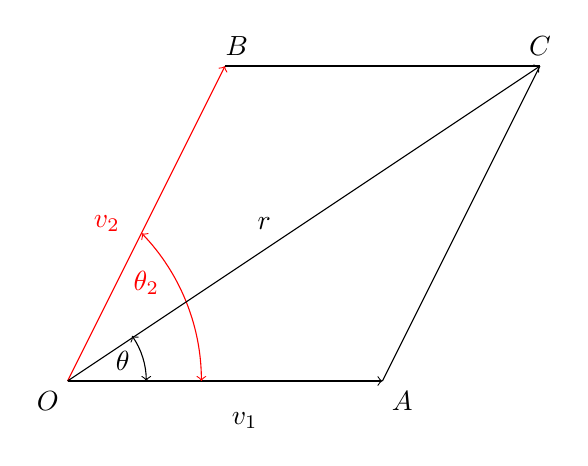
\begin{tikzpicture}
%the vectors
\draw [->, black] (1.0,0) -- (5.0,0.0);
\draw [black] (3.25, -0.5) node [black]{$v_1$};

\draw [->, red] (1.0,0) -- (3.0,4.0);
\draw (1.5, 2.0) node [red]{$v_2$}; 
\draw [red, <->] (2.7,0) arc (0:44:2.7); 
\draw (2., 1.25) node [red]{$\theta_2$};

%the shadow
\draw [-, black] (5.0, 0,0) -- (7.0,4.0);
\draw [-, black] (3.0,4.0) -- (7.0,4.0);

%the resultant
\draw [->, black] (1.0,0) -- (7.0,4.0);
\draw [black] (3.5, 2.0) node [black]{$r$}; 
\draw [black, <->] (2.0,0) arc (0:35:1);
\draw (1.7, .25) node {$\theta$};

\draw [black] (.75, -.25) node {$O$}; 
\draw [black] (5.25, -.25) node {$A$}; 
\draw [black] (3.15, 4.25) node {$B$};
\draw [black] (7.0, 4.25) node {$C$}; 
\end{tikzpicture}

Dengan $r$, $v_1$, $\theta$ diketahui, carilah nilai $\theta_2$ dan $v_2$ ($OB$)!

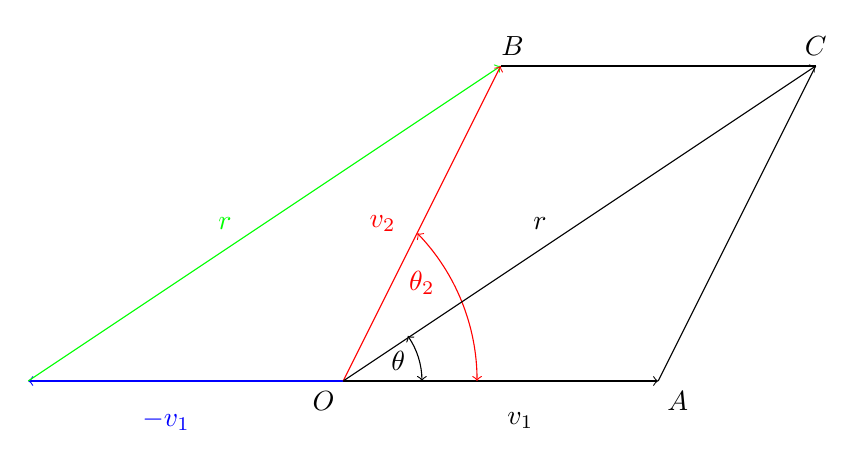
\begin{tikzpicture}
%the vectors
\draw [->, black] (1.0,0) -- (5.0,0.0);
\draw [black] (3.25, -0.5) node [black]{$v_1$};

\draw [->, blue] (1.0,0) -- (-3.0,0.0);
\draw (-1.25, -0.5) node [blue]{$-v_1$};

\draw [->, green] (-3.0,0) -- (3.0,4.0);
\draw [green] (-.5, 2.0) node {$r$}; 

\draw [->, red] (1.0,0) -- (3.0,4.0);
\draw (1.5, 2.0) node [red]{$v_2$}; 
\draw [red, <->] (2.7,0) arc (0:44:2.7); 
\draw (2., 1.25) node [red]{$\theta_2$};

%the shadow
\draw [-, black] (5.0, 0,0) -- (7.0,4.0);
\draw [-, black] (3.0,4.0) -- (7.0,4.0);

%the resultant
\draw [->, black] (1.0,0) -- (7.0,4.0);
\draw [black] (3.5, 2.0) node [black]{$r$}; 
\draw [black, <->] (2.0,0) arc (0:35:1);
\draw (1.7, .25) node {$\theta$};

\draw [black] (.75, -.25) node {$O$}; 
\draw [black] (5.25, -.25) node {$A$}; 
\draw [black] (3.15, 4.25) node {$B$}; 
\draw [black] (7.0, 4.25) node {$C$}; 
\end{tikzpicture}

Garis $OB$ sama dengan diagonal jajaran genjang yang dibentuk oleh
$OC$ dan $OA$ dibalik.

$v_2$ atau $OB$ adalah:

\begin{align*}
v_2 &= \sqrt{(-v_1)^2 + r^2 + 2v_1r\cos(\pi - \theta_2)}\\
v_2 &= \sqrt{v_1^2 + r^2 - 2v_1r\cos\theta_2}\\
\end{align*}

$\theta_2$ is

\begin{align*}
\theta_2 &= \frac{r\sin\theta}{-v_1 + r\cos\theta}
\end{align*}

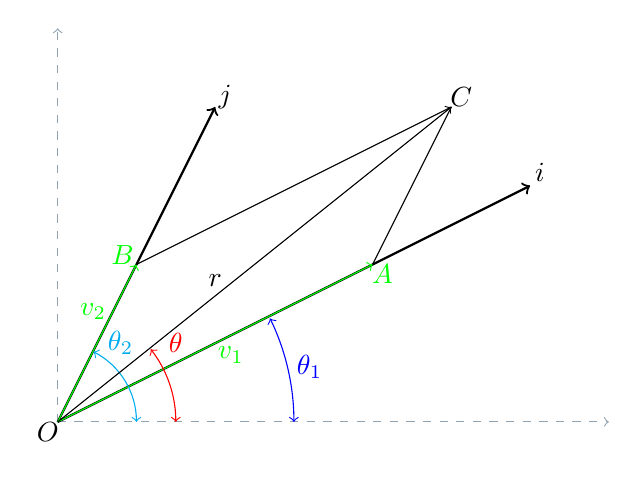
\begin{tikzpicture}
%common point
\draw [black] (0.875, -0.125) node {$O$};
%the vectors
\draw [dashed, ->, cadetgrey] (1.0,0.0) -- (8.0,0.0);
\draw [dashed, ->, cadetgrey] (1.0,0.0) -- (1.0,5.0);

\draw [thick, ->, black] (1.0,0.0) -- (7.0,3.0);
\draw [black] (7.125, 3.175) node {$i$};
\draw [->, green] (1.0,0) -- (5.0,2.0);
\draw [green] (5.125, 1.875) node {$A$};
\draw (4.2, 0.7) node [blue]{$\theta_1$};
\draw [dotted] (3.2, 0.85) node [green]{$v_1$};
\draw [blue, <->] (4.0,0) arc (0:26:3.0); 

\draw [thick, ->, black] (1.0,0) -- (3.,4.0);
\draw [black] (3.125, 4.125) node {$j$};
\draw [->, green] (1.0,0) -- (2.0,2.0);
\draw [green] (1.825, 2.125) node {$B$};
\draw [dotted] (1.45, 1.4) node [green]{$v_2$};
\draw [dotted] (1.8, 1.) node [cyan]{$\theta_2$};
\draw [cyan, <->] (2.0,0) arc (0:63:1.); 

%the shadow
\draw [-, black] (5.0, 2,0) -- (6.0,4.0);
\draw [-, black] (2.0,2.0) -- (6.0,4.0);
%the resultant
\draw [->, black] (1.0,0) -- (6.0,4.0);
\draw [black] (6.125, 4.125) node {$C$};
\draw [dotted] (3, 1.8) node [black]{$r$};
\draw (2.5, 1.) node [red]{$\theta$};
\draw [red, <->] (2.5,0) arc (0:38:1.5); 
\end{tikzpicture}

 \begin{align*}
v_1 + v_2\cos (\theta_2 - \theta_1) &= r \cos(\theta - \theta_1)\\
v_1 \cos(\theta_2 - \theta_1) + v_2 &= r \cos(\theta_2 - \theta)\\
\end{align*}

so

\begin{align*}
v_1 + v_2\cos (\theta_2 - \theta_1) &= r \cos(\theta - \theta_1)\\
v_1 \cos(\theta_2 - \theta_1)\cos(\theta_2 - \theta_1) + v_2 \cos(\theta_2 - \theta_1) &= r \cos(\theta_2 - \theta) \cos(\theta_2 - \theta_1)\\
v_1(1 - \cos^2(\theta_2 - \theta_1)) &= r(\cos(\theta - \theta_1) - \cos(\theta_2 - \theta)\cos(\theta_2 - \theta_1) )\\
v_1 &= r\frac{(\cos(\theta - \theta_1) - \cos(\theta_2 - \theta)\cos(\theta_2 - \theta_1) )}{(1 - \cos^2(\theta_2 - \theta_1))}\\
\end{align*}

%\begin{tikzpicture} 
%% Draw the first line with absolute coordinates and the 
%% second with relative coordinates to the first line
%\draw (0,0) -- (30:3cm) -- ++(80:3cm); 
%\end{tikzpicture}

example let :

$100/60^\circ, 30^\circ, 60^\circ$

\begin{tikzpicture} 
%\draw (0,0) -- (10:3) -- ++(30:3); 
\draw (0,0) -- (30:5.77) -- ++(90:5.77);
\draw (0,0) -- (60:10);
\draw (0,0) -- (90:5.77) -- ++(30:5.77);
\draw (2.7, 1.2) node [blue] {$v_1$};
\draw (2.7, 4.2) node [black] {$r$};
\draw (-.5, 3.5) node [blue] {$v_2$};
\draw [dashed, cadetgrey, ->](0,0) -- (90:8);
\draw [dashed, cadetgrey, ->](0,0) -- (0:8);
\draw [black, <->] (.5,0) arc (0:90:.5); 
\draw [black] (.20, 1) node {\rotatebox{90}{$90^\circ$}};
\draw [black] (.65, .70) node {\rotatebox{60}{$60^\circ$}};
\draw [black] (1., .25) node {\rotatebox{30}{$30^\circ$}};
\end{tikzpicture}

\begin{align*}
v_1 &= r\frac{\cos(\theta - \theta_1) - \cos(\theta_2 - \theta)\cos(\theta_2 - \theta_1) }{(1 - \cos^2(\theta_2 - \theta_1))}\\
v_1 &= 100\frac{\cos(60^\circ-30^\circ) - \cos(90^\circ - 60^\circ)\cos(90^\circ - 30^\circ)}{1 - \cos^2(90^\circ - 30^\circ)}\\
v_1 &= 100\frac{\cos(30^\circ) - \cos(30^\circ)\cos(60^\circ)}{1 \cos^2(60^\circ)}\\
v_1 &= 100\frac{\cos(30^\circ)(1-cos(60^\circ))}{1-\cos^2(60^\circ)}\\
v_1 &= 100\frac{\cos(30^\circ)(1-\cos(60^\circ))}{(1-\cos(60^\circ))(1+\cos(60^\circ))}\\
v_1 &= 100\frac{\cos(30^\circ)}{1+\cos(60^\circ)}\\
\end{align*}

Komposisi beberapa vektor dengan titik awal bersama. $Resultant$ nya dapat 
diperoleh dengan konstruksi grafix berikut: Ambil vektor dengan sembarang 
urutan, misal $A$, $B$, $C$. Dari titik akhir $A$ gambarkan $\grave{B}$ yang 
sama panjang dan paralel dengan $B$, dan dari titik akhir $\grave{B}$ tarik 
vektor $\grave{C}$ yang sama panjang dan paralel dengan $C$. Vektor yang 
bermula dari $A$ dan berakhir di $\grave{C}$ adalah $Resultant$ dari 
vektor - vektor tersebut. $Resultant$ yang didapat sama tanpa memperhatikan 
urutan vektor, dan karena urutannya tidak menentukan area yang diliputi.

Hasilnya dapat di peroleh secara analitis sebagai berikut.
Misalkan 
\[
f_1/\underline{\theta_1} + f_2/\underline{\theta_2} +  ... + f_n/\underline{\theta_n}.
\]
sekarang
\[
f_1/\underline{\theta_1} = f_1\cos\theta_1/\underline{0} + f_1\sin\theta_1/\underline{\frac{\pi}{2}} 
\]
juga
\[
f_2/\underline{\theta_2} = f_2\cos\theta_2/\underline{0} + f_2\sin\theta_2/\underline{\frac{\pi}{2}} 
\]
dan
\[
f_n/\underline{\theta_n} = f_n\cos\theta_n/\underline{0} + f_n\sin\theta_n/\underline{\frac{\pi}{2}} 
\]
dengan demikian
\begin{align*}
\sum\Bigl\lbrace f/\theta \Bigr\rbrace &= \Bigl\lbrace \sum{f \cos\theta}\Bigr\rbrace/0 + \Bigl\lbrace\sum{f \sin\theta}\Bigr\rbrace/\frac{\pi}{2}\\
&=\sqrt{(\sum{f \cos\theta})^2 + (\sum{f \sin \theta})^2}/\tan^{-1}\frac{\sum f \sin \theta}{\sum f \cos \theta}
\end{align*}

Quaternion
\begin{align*}
(\alpha_1, 0) (a_1, a_2) &= (\alpha_1 a_1, \alpha_1 a_2)\\
(\alpha_1, \alpha_2) (a_1, 0) &= (\alpha_1 a_1, \alpha_2 a_1)\\
(0, \alpha_2)(0, a_2) &= (-1 \alpha_2 a_2, 0 \alpha_2 a_2)\\
(\alpha_1, \alpha_2) &= (\alpha_1, 0) + (0, \alpha_2)\\
(\alpha_1, \alpha_2) (a_1, a_2) &= (\alpha_1, 0)(a_1, a_2) + (0, \alpha_2)(a_1, a_2)\\
(\alpha_1, \alpha_2) (a_1, a_2) &= (\alpha_1 a_1, \alpha_1 a_2) + (0, \alpha_2)(a_1, a_2)\\
(\alpha_1, \alpha_2) (a_1, a_2) &= (\alpha_1 a_1, \alpha_1 a_2) + (0, \alpha_2)(0, a_2) + (0, \alpha_2)(a_1, 0)\\
(\alpha_1, \alpha_2) (a_1, a_2) &= (\alpha_1 a_1, \alpha_1 a_2) + (-\alpha_2 a_2, 0) + (0, \alpha_2)(a_1, 0)\\
(\alpha_1, \alpha_2) (a_1, a_2) &= (\alpha_1 a_1, \alpha_1 a_2) + (-\alpha_2 a_2, 0) + (a_1 0, a_1 \alpha_2)\\
(\alpha_1, \alpha_2) (a_1, a_2) &= (\alpha_1 a_1 -\alpha_2 a_2 , \alpha_1 a_2 + \alpha_2 a_1)
\end{align*}

Quaternion15
\begin{align*}
(0, 1)(a, b) &= (0, 1)(a, 0) + (0, 1)(0, b)\\
(0, 1)(a, b) &= (0, a) + (-b, 0)\\
(0, 1)(a, b) &= (-b, a)
\end{align*}

Examples To Try
\begin{align*}
(4 + 3i)\cdot i &=  4i -3\\
(4 + 3i)\cdot 2i &=  8i -6\\
(4 + 3i)\cdot (4 + 3i) &=  16 + 12i + 12i + 9i^2\\
&= 16 + 24i -9\\
&= 7 + 24i\\
(2 + i)(1 + 2i) &= 2 + 5i -2\\
&= 5i
\end{align*} 


\textbf{del Ferro - Cardan - Bombelli}

Solutions to quadration equation

\begin{align*}
ax^2 + bx + c &= 0\\
ax^2 &= -bx - c\\
ax^2 &= -bx - c\\
\frac{ax^2}{b} &= -\frac{bx}{b} - \frac{c}{b}\\ 
\frac{a}{b}x\times x + x&= -\frac{c}{b}
\end{align*}

\end{document}
